\documentclass[]{article}
\usepackage[UTF8]{ctex}
\usepackage{graphicx}
\usepackage{appendix}
\usepackage{geometry}
\usepackage{amsmath}
\usepackage{cite}
\usepackage{natbib}
\usepackage{listings}
\usepackage{titlesec}
\usepackage{float}
\usepackage{enumitem}
\usepackage[labelfont=bf]{caption}
\usepackage{listings}
\usepackage{hyperref}  
\usepackage[section]{placeins}
\usepackage{fix-cm}
\hypersetup{hidelinks,
	colorlinks=true,
	allcolors=black,
	pdfstartview=Fit,
	breaklinks=true
}

\lstset{
    basicstyle=\ttfamily,
    breaklines=true,
    frame=single,
    numbers=left,
    numberstyle=\tiny,
    language=[LaTeX]TeX
}

% Set ctex labels to English
\ctexset{
    contentsname = {Contents},
    figurename = {Figure},
    tablename = {Table},
    appendixname = {Appendix},
    abstractname = {Abstract},
    indexname = {Index},
    proofname = {Proof}
}

\begin{document}

\title{\huge Design of a vending machine}
\author{\large }
\date{}

\maketitle

\vspace{3cm}

\begin{center}
    {\large
        \begin{tabular}{|p{2.5cm}|p{3.5cm}|p{2.5cm}|p{3.5cm}|}
            \hline
            \textbf{Name}     &  & \textbf{Class} &       \\[0.8cm]
            \hline
            \textbf{Date}     &  & \textbf{Score} & \quad \\[0.8cm]
            \hline
            \textbf{Examiner} &  & \quad          & \quad \\[0.8cm]
            \hline
        \end{tabular}
    }
\end{center}

\newpage
\tableofcontents
\newpage
\newpage

\section{Introduction}
A 4-bit vending machine system is designed to manage the sale of items with a price of 5 yuan. The system employs a finite state machine architecture to handle different payment scenarios, including accepting 5-yuan notes directly or four 1-yuan coins. This hierarchical design allows for efficient and modular implementation of state-based control on FPGA platforms. The experiment focuses on implementing and simulating this vending machine system using VHDL on Quartus II and ModelSim tools.

\section{Experiment procedure}

\subsection{Set Up the Project}

\begin{enumerate}[label = (\arabic*)]
    \item Launch Quartus II 13.0 software.
    \item Open Quartus II software and create a new project using the "New Project Wizard." Name the project as vending\_machine and configure the project folder and top-level entity details.
    \item For device selection, if only simulation is required, allow Quartus II to auto-select the default FPGA device.

\end{enumerate}


\subsection{Design the Components}
\noindent The vending machine system consists of a finite state machine that manages payment processing and item dispensing based on customer input. The design follows a state-based approach to handle various payment scenarios.

\begin{figure}[H]
    \centering
    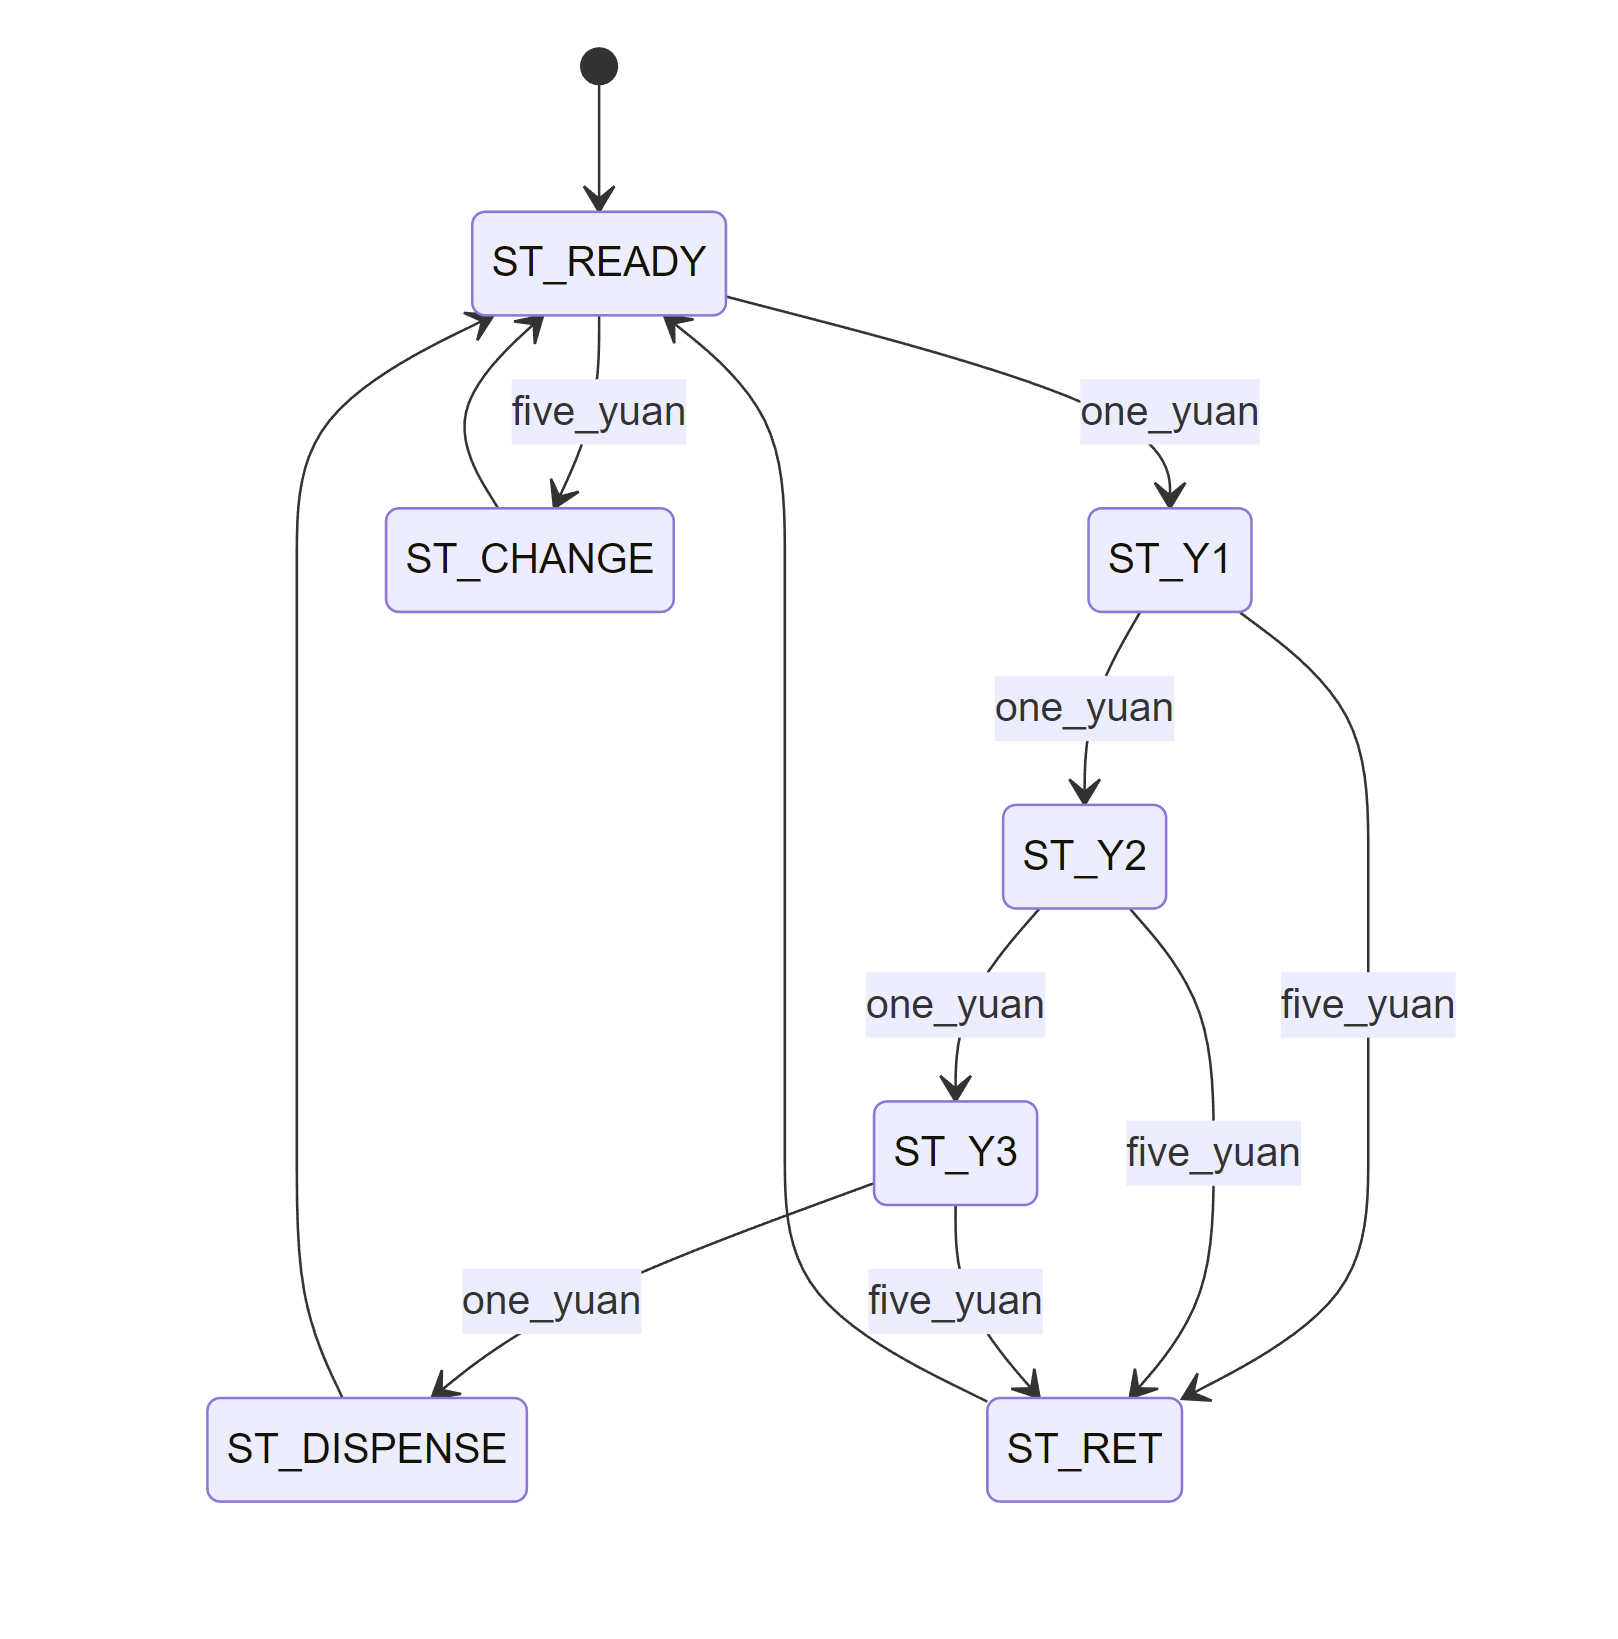
\includegraphics[width=0.8\linewidth]{fsm.jpg}
    \caption{State diagram of the vending machine}
    \label{fig:state-diagram}
\end{figure}

\noindent We follow these steps to implement the vending machine:

\begin{lstlisting}[language = VHDL]
library ieee;
use ieee.std_logic_1164.all;

entity vending_machine is
    port(
        clk           : in  std_logic;
        rst           : in  std_logic;
        one_yuan      : in  std_logic;
        five_yuan     : in  std_logic;

        ready         : out std_logic;
        cash          : out std_logic;
        output_ticket : out std_logic;
        give_charge   : out std_logic;
        retmoney      : out std_logic
    );
end vending_machine;

architecture fsm of vending_machine is

    type state_type is (
        ST_READY, ST_Y1, ST_Y2, ST_Y3,
        ST_DISPENSE, ST_CHANGE, ST_RET
    );

    signal state, next_state : state_type;

begin

    process(clk, rst)
    begin
        if rst = '1' then
            state <= ST_READY;
        elsif rising_edge(clk) then
            state <= next_state;
        end if;
    end process;

    process(state, one_yuan, five_yuan)
    begin
        next_state <= state;

        case state is

            when ST_READY =>
                if five_yuan = '1' then
                    next_state <= ST_CHANGE;
                elsif one_yuan = '1' then
                    next_state <= ST_Y1;
                end if;

            when ST_Y1 =>
                if five_yuan = '1' then
                    next_state <= ST_RET;
                elsif one_yuan = '1' then
                    next_state <= ST_Y2;
                end if;

            when ST_Y2 =>
                if five_yuan = '1' then
                    next_state <= ST_RET;
                elsif one_yuan = '1' then
                    next_state <= ST_Y3;
                end if;

            when ST_Y3 =>
                if five_yuan = '1' then
                    next_state <= ST_RET;
                elsif one_yuan = '1' then
                    next_state <= ST_DISPENSE;
                end if;

            when ST_DISPENSE =>
                next_state <= ST_READY;

            when ST_CHANGE =>
                next_state <= ST_READY;

            when ST_RET =>
                next_state <= ST_READY;

            when others =>
                next_state <= ST_READY;

        end case;
    end process;

    process(state)
    begin
        ready         <= '0';
        cash          <= '0';
        output_ticket <= '0';
        give_charge   <= '0';
        retmoney      <= '0';

        case state is
            when ST_READY =>
                ready <= '1';

            when ST_Y1 | ST_Y2 | ST_Y3 =>
                cash <= '1';

            when ST_DISPENSE =>
                output_ticket <= '1';

            when ST_CHANGE =>
                output_ticket <= '1';
                give_charge   <= '1';

            when ST_RET =>
                retmoney <= '1';

            when others =>
                null;
        end case;
    end process;

end fsm;

\end{lstlisting}

\begin{figure}[H]
    \centering
    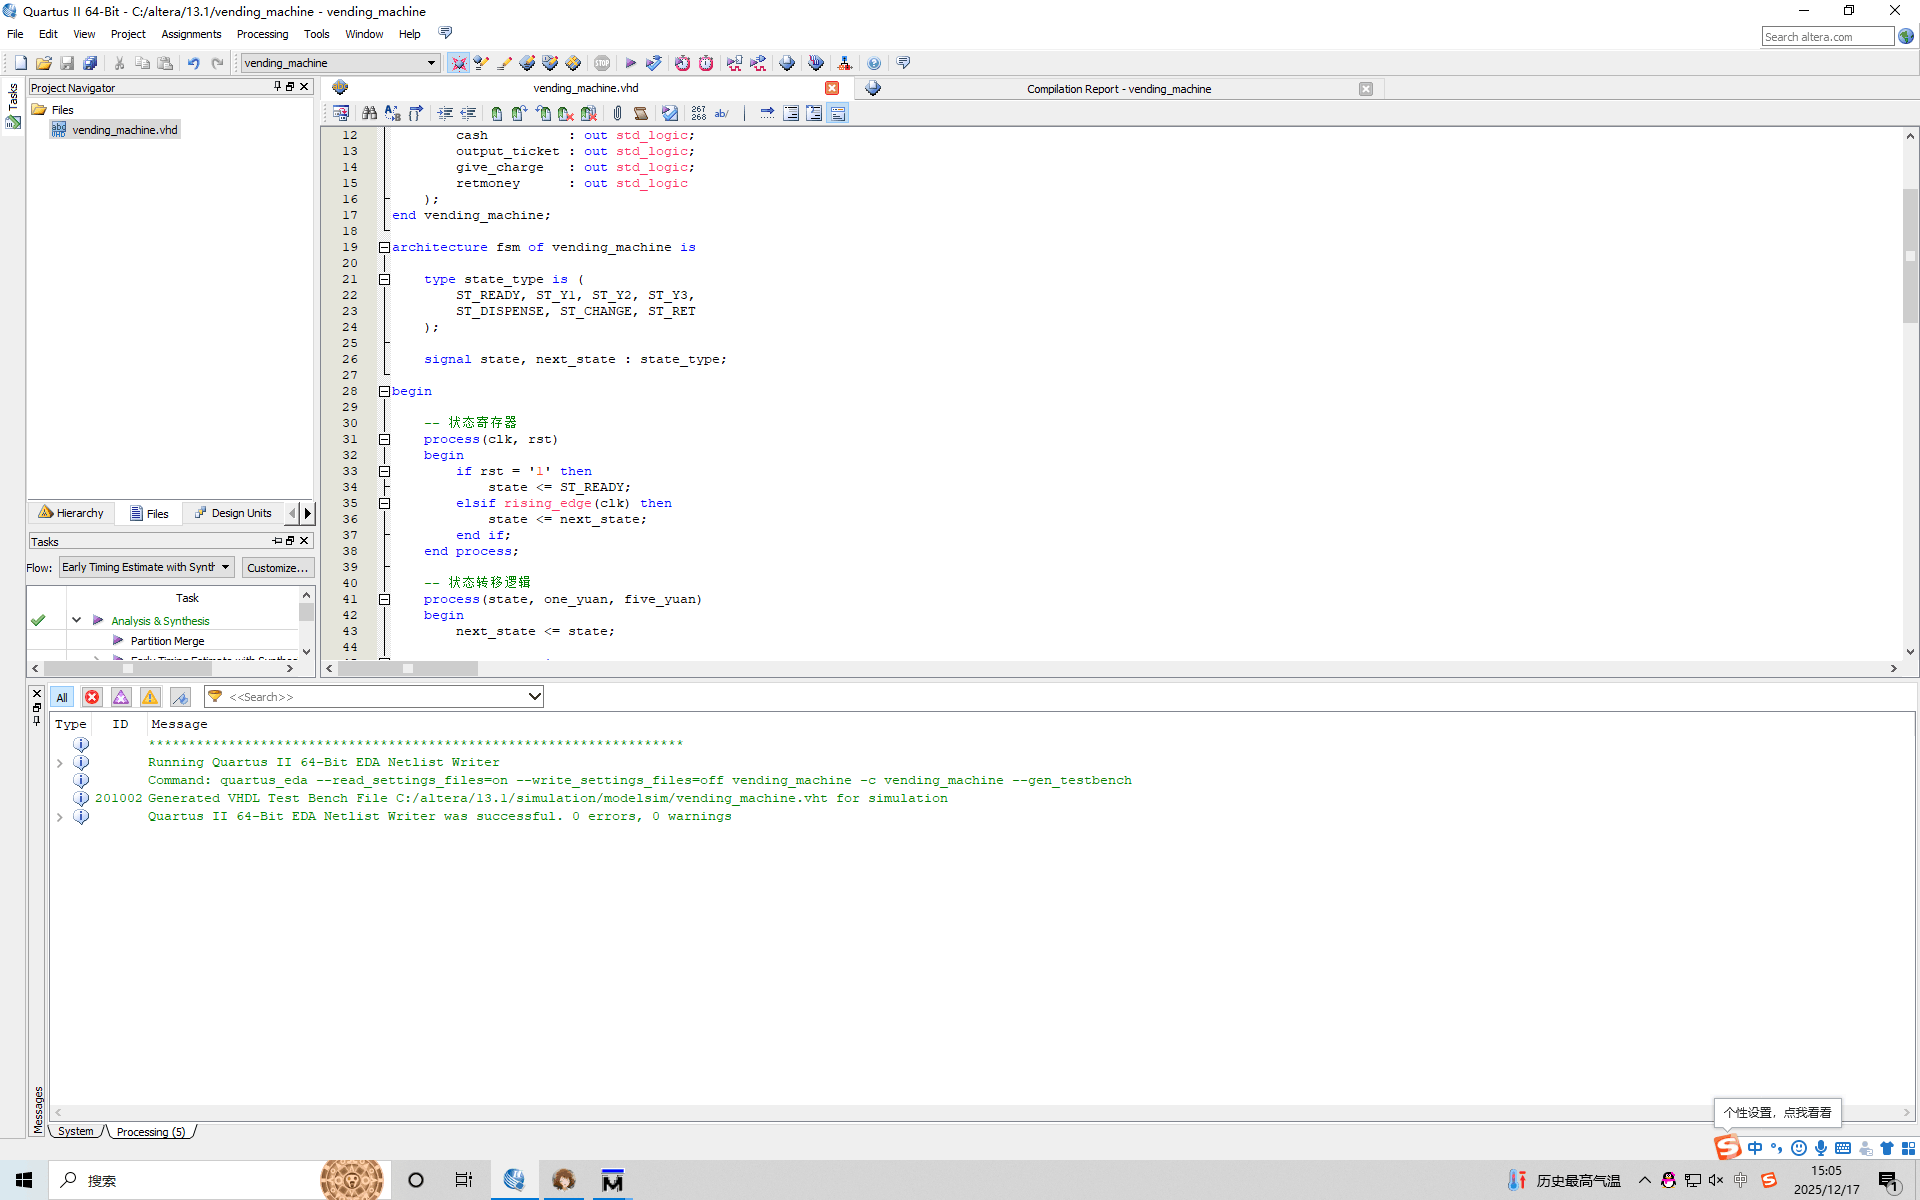
\includegraphics[width=1\linewidth]{vhd.png}
    \caption{Vending Machine FSM Implementation}
    \label{fig:vending-machine-impl}
\end{figure}

\subsection{Testbench Design}
\renewcommand{\theenumi}{(\arabic{enumi})}
\begin{enumerate}
    \item Create a testbench file named vending\_machine\_testbench.vhd.
    \item Design the testbench to test the following scenarios:
          \begin{enumerate}
              \item Give the machine a 5-yuan cash when it is ready.
              \item Give the machine four 1-yuan cash when it is ready.
              \item Give the machine two 1-yuan cash and then a 5-yuan cash when it is ready.
          \end{enumerate}
    \item Add appropriate clock and signal initialization to simulate the system's behavior.
    \item Compile the testbench to verify its functionality.
\end{enumerate}

\begin{lstlisting}[language = VHDL]
library ieee;
use ieee.std_logic_1164.all;

entity vending_machine_tb is
end vending_machine_tb;

architecture sim of vending_machine_tb is

    signal clk           : std_logic := '0';
    signal rst           : std_logic := '1';
    signal one_yuan      : std_logic := '0';
    signal five_yuan     : std_logic := '0';

    signal ready         : std_logic;
    signal cash          : std_logic;
    signal output_ticket : std_logic;
    signal give_charge   : std_logic;
    signal retmoney      : std_logic;

begin

    uut: entity work.vending_machine
        port map(
            clk           => clk,
            rst           => rst,
            one_yuan      => one_yuan,
            five_yuan     => five_yuan,
            ready         => ready,
            cash          => cash,
            output_ticket => output_ticket,
            give_charge   => give_charge,
            retmoney      => retmoney
        );

    clk <= not clk after 5 ns;

    process
    begin
        -- reset
        rst <= '1';
        wait for 20 ns;
        rst <= '0';

        wait for 20 ns;
        five_yuan <= '1';
        wait for 10 ns;
        five_yuan <= '0';

        wait for 40 ns;

        one_yuan <= '1'; wait for 10 ns; one_yuan <= '0';
        wait for 10 ns;
        one_yuan <= '1'; wait for 10 ns; one_yuan <= '0';
        wait for 10 ns;
        one_yuan <= '1'; wait for 10 ns; one_yuan <= '0';
        wait for 10 ns;
        one_yuan <= '1'; wait for 10 ns; one_yuan <= '0';

        wait for 40 ns;

        one_yuan <= '1'; wait for 10 ns; one_yuan <= '0';
        wait for 10 ns;
        one_yuan <= '1'; wait for 10 ns; one_yuan <= '0';
        wait for 10 ns;

        five_yuan <= '1'; wait for 10 ns; five_yuan <= '0';

        wait for 50 ns;
        wait;
    end process;

end sim;


\end{lstlisting}

\begin{figure}[H]
    \centering
    
\includegraphics[width=1\linewidth]{vht.png}
    \caption{Testbench Code}
    \label{fig:testbench}
\end{figure}

\subsection{Simulation}
\begin{enumerate}
    \item Open ModelSim and set up the simulation environment.
    \item Add the compiled vending machine system and its testbench files to the ModelSim project.
    \item Simulate the design by applying all test cases through the testbench. Observe the output waveforms for each input combination.
    \item Record the simulation waveforms and save the results for inclusion in the report.
\end{enumerate}


\section{Experimental record}

\noindent Below are some experimental records from the vending machine simulation.

\begin{figure}[H]
    \centering
    
\includegraphics[width=1\linewidth]{wave.png}
    \caption{Simulation Waveform}
    \label{fig:waveform}
\end{figure}

\section{Analysis and discussion}
\subsection{Overall Conclusion}
\noindent The simulation waveform confirms the correct operation of the vending machine's finite state machine. Key observations include:

\begin{enumerate}
    \item The system correctly initializes to the \textbf{ST\_READY} state upon receiving a high \texttt{rst} signal.
    \item The state transitions respond accurately to the input signals \texttt{one\_yuan} and \texttt{five\_yuan}:
          \begin{itemize}
              \item A 1-yuan input (\texttt{one\_yuan = 1}) transitions the system through the states \texttt{ST\_Y1}, \texttt{ST\_Y2}, and \texttt{ST\_Y3}, where four consecutive inputs are required to dispense a ticket.
              \item A 5-yuan input (\texttt{five\_yuan = 1}) in the ready state transitions the system to \texttt{ST\_CHANGE}, where a ticket is dispensed and change is given.
          \end{itemize}
    \item The output signals \texttt{output\_ticket}, \texttt{give\_charge}, and \texttt{retmoney} are asserted at the correct times, matching the expected behavior for each state.
    \item The \texttt{retmoney} signal is asserted in the \textbf{ST\_RET} state, ensuring the system handles invalid input conditions gracefully (e.g., inserting a 5-yuan input while waiting for consecutive 1-yuan inputs).
\end{enumerate}

\noindent In general, the finite state machine design operates as intended, validating the logical flow of states and the corresponding outputs. The system successfully meets the functional requirements for a simple vending machine.

\subsection{Function of the System}
\begin{enumerate}
    \item The \textbf{ST\_READY} state waits for customer input and outputs the \texttt{ready} signal.
    \item The \textbf{ST\_Y1}, \textbf{ST\_Y2}, and \textbf{ST\_Y3} states accumulate consecutive 1-yuan inputs, requiring four such inputs to dispense a ticket.
    \item The \textbf{ST\_CHANGE} state processes a 5-yuan payment by dispensing a ticket and providing change.
    \item The \textbf{ST\_DISPENSE} state outputs the \texttt{output\_ticket} signal to dispense the ticket.
    \item The \textbf{ST\_RET} state returns all inserted money and then transitions back to the \textbf{ST\_READY} state.
\end{enumerate}

\subsection{Waveform Analysis}
\noindent The simulation waveform demonstrates the behavior of the vending machine under various input conditions:

\begin{enumerate}
    \item \textbf{Inserting 5-yuan:}
          \begin{itemize}
              \item When \texttt{five\_yuan = 1} in the \textbf{ST\_READY} state, the system transitions to \textbf{ST\_CHANGE}.
              \item The \texttt{give\_charge} signal is asserted, indicating that change is being dispensed.
              \item The \texttt{output\_ticket} signal is asserted, indicating that a ticket is issued.
              \item After completing these actions, the system returns to the \textbf{ST\_READY} state.
          \end{itemize}

    \item \textbf{Inserting four consecutive 1-yuan inputs:}
          \begin{itemize}
              \item When \texttt{one\_yuan = 1}, the \texttt{cash} signal remains high, indicating that the system is accumulating inserted cash.
              \item After four consecutive 1-yuan inputs, the state transitions to \textbf{ST\_DISPENSE}.
              \item The \texttt{output\_ticket} signal is asserted, indicating that a ticket is issued.
              \item The system then returns to the \textbf{ST\_READY} state.
          \end{itemize}

    \item \textbf{Inserting two 1-yuan inputs followed by an incorrect 5-yuan input:}
          \begin{itemize}
              \item The system initially transitions through \textbf{ST\_Y1} and \textbf{ST\_Y2} as two 1-yuan inputs are received.
              \item When a 5-yuan input (\texttt{five\_yuan = 1}) is detected during this process, the system identifies an invalid input sequence.
              \item The state transitions to \textbf{ST\_RET}, and the \texttt{retmoney} signal is asserted, indicating that all inserted money is being refunded.
              \item The system then returns to the \textbf{ST\_READY} state.
          \end{itemize}
\end{enumerate}

\end{document}
